\begin{appendices}

    \chapter{Gestion de projet}\label{ch-a:gestion-projet}

    \section[Jira : L'outil pour la gestion de projet]{Jira : L'outil essentiel pour la gestion quotidienne de projet}\label{sec-a:jira}

    \begin{figure}[ht]
        \centering
        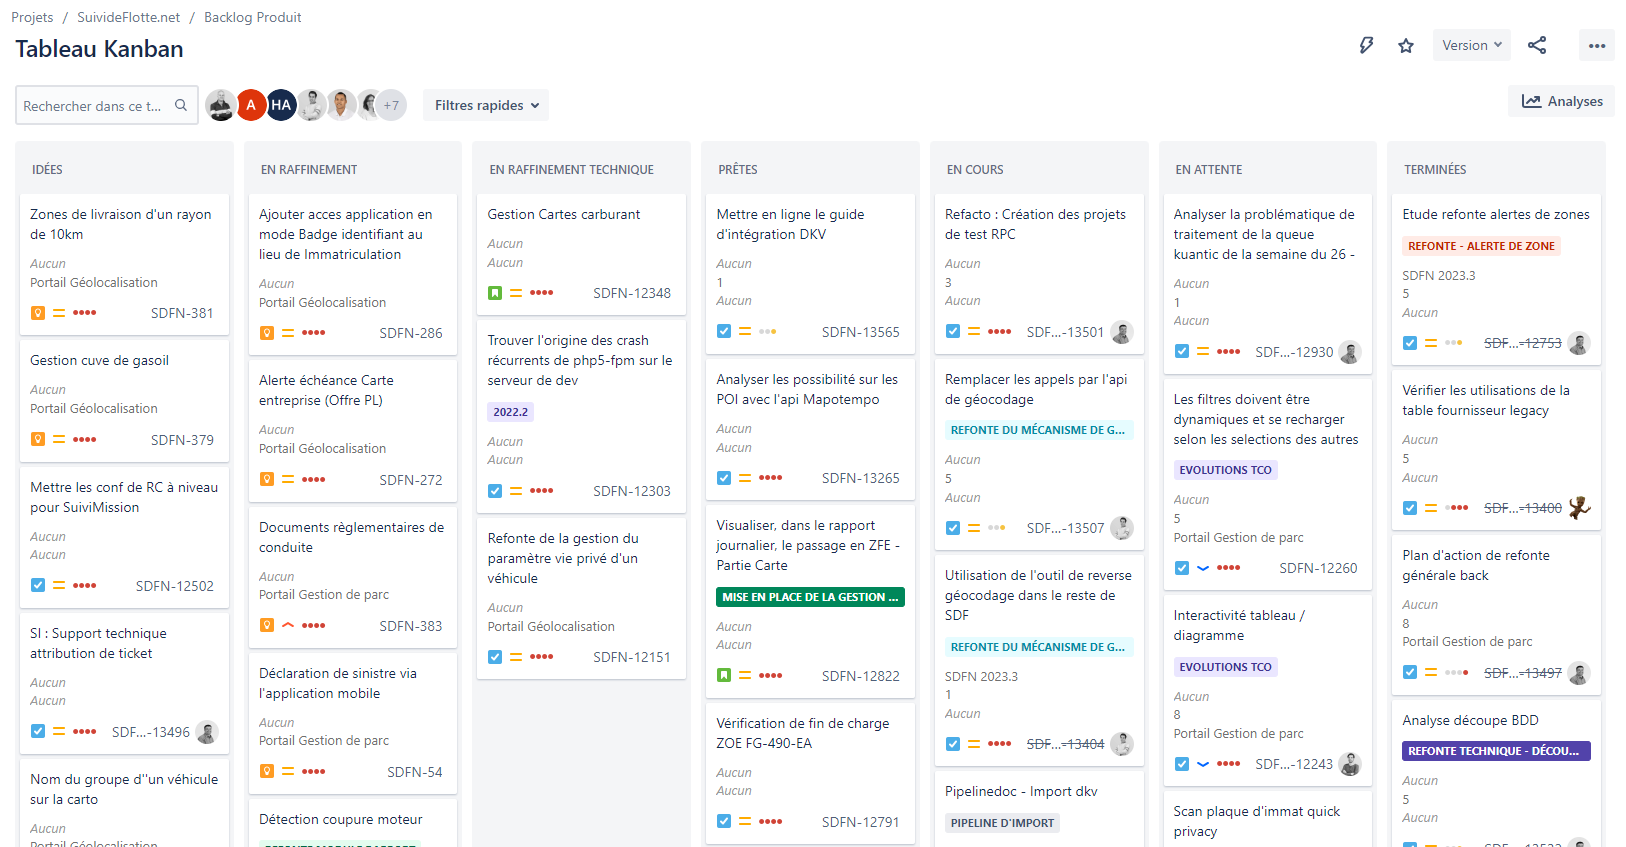
\includegraphics[width=\textwidth]{img/product-backlog}
        \caption{Le Backlog de produit sous forme de tableau Kanban dans Jira.}
        \label{fig:product-backlog}
    \end{figure}

    \begin{figure}[ht]
        \centering
        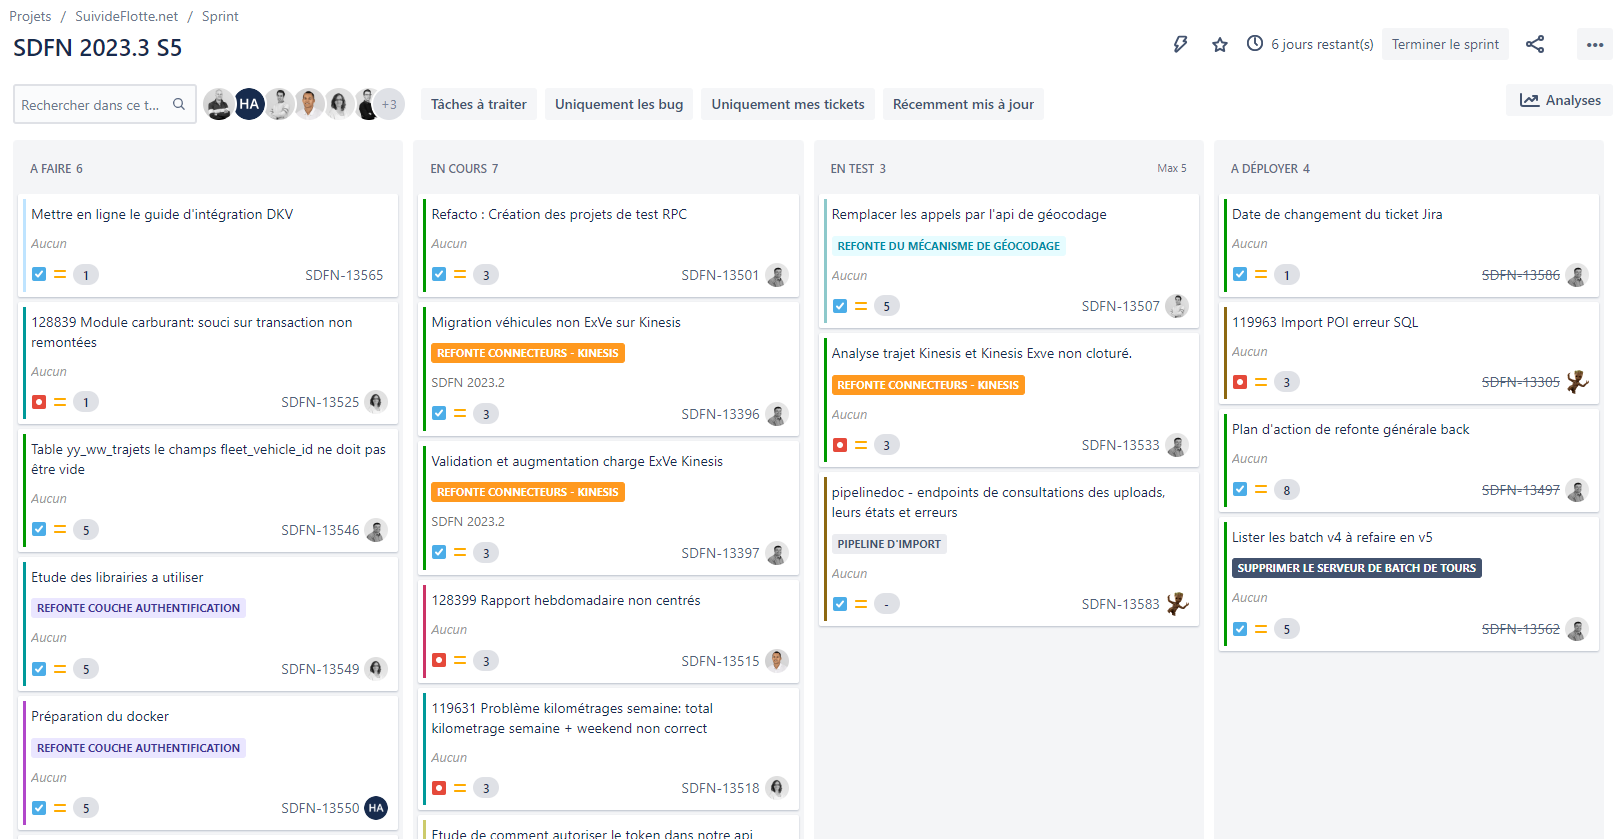
\includegraphics[width=\textwidth]{img/sprint}
        \caption{Le Backlog de sprint sous forme de tableau Kanban dans Jira.}
        \label{fig:sprint-backlog}
    \end{figure}

    \begin{figure}[ht]
        \centering
        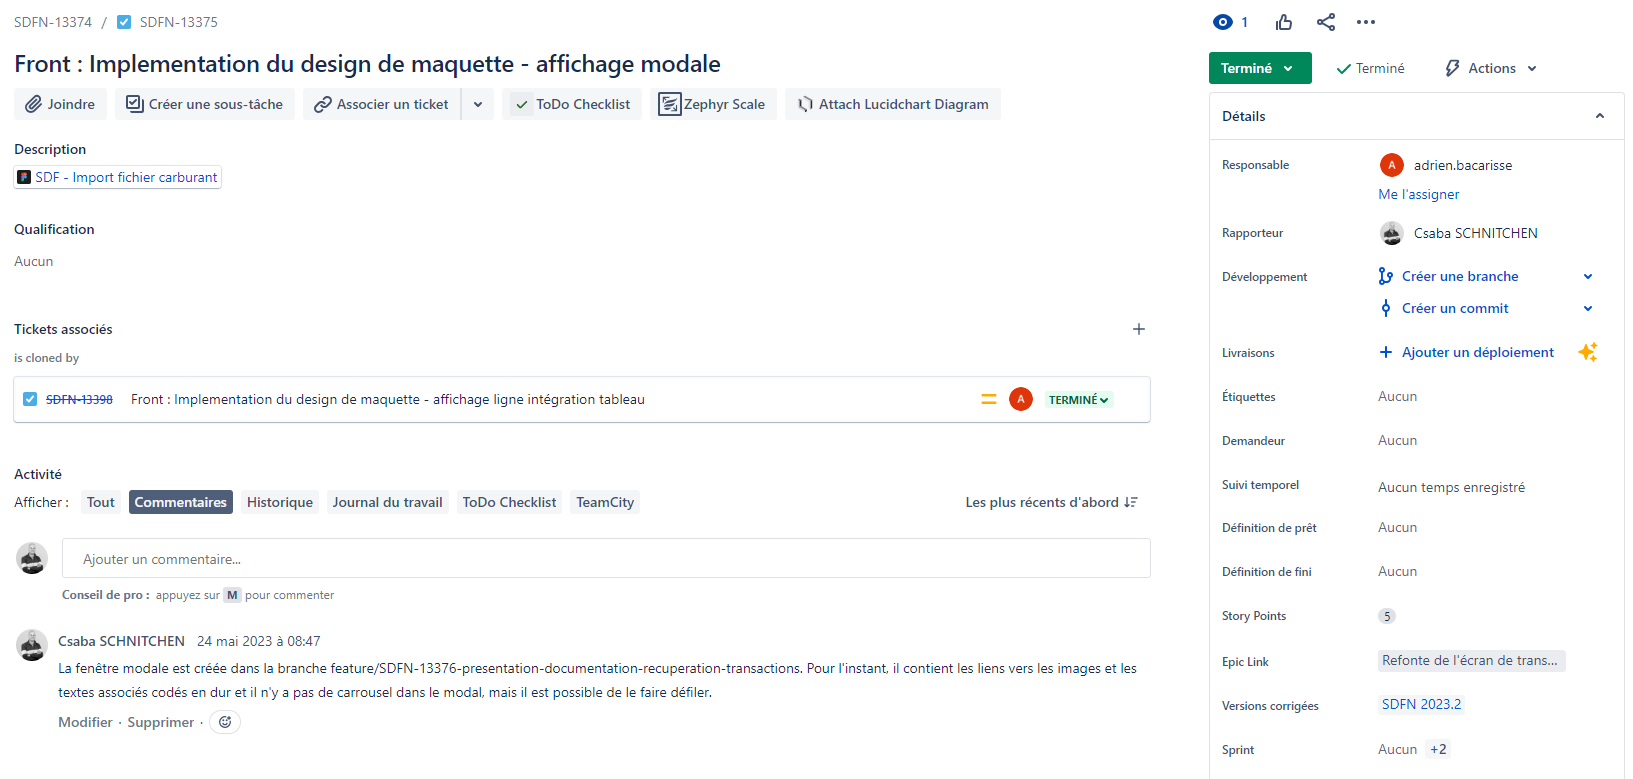
\includegraphics[width=\textwidth]{img/ticket}
        \caption{Un exemple de ticket dans Jira pour le projet d'amélioration de la page d'importation des fichiers des transactions de carburant.}
        \label{fig:ticket}
    \end{figure}

    \begin{figure}[ht]
        \centering
        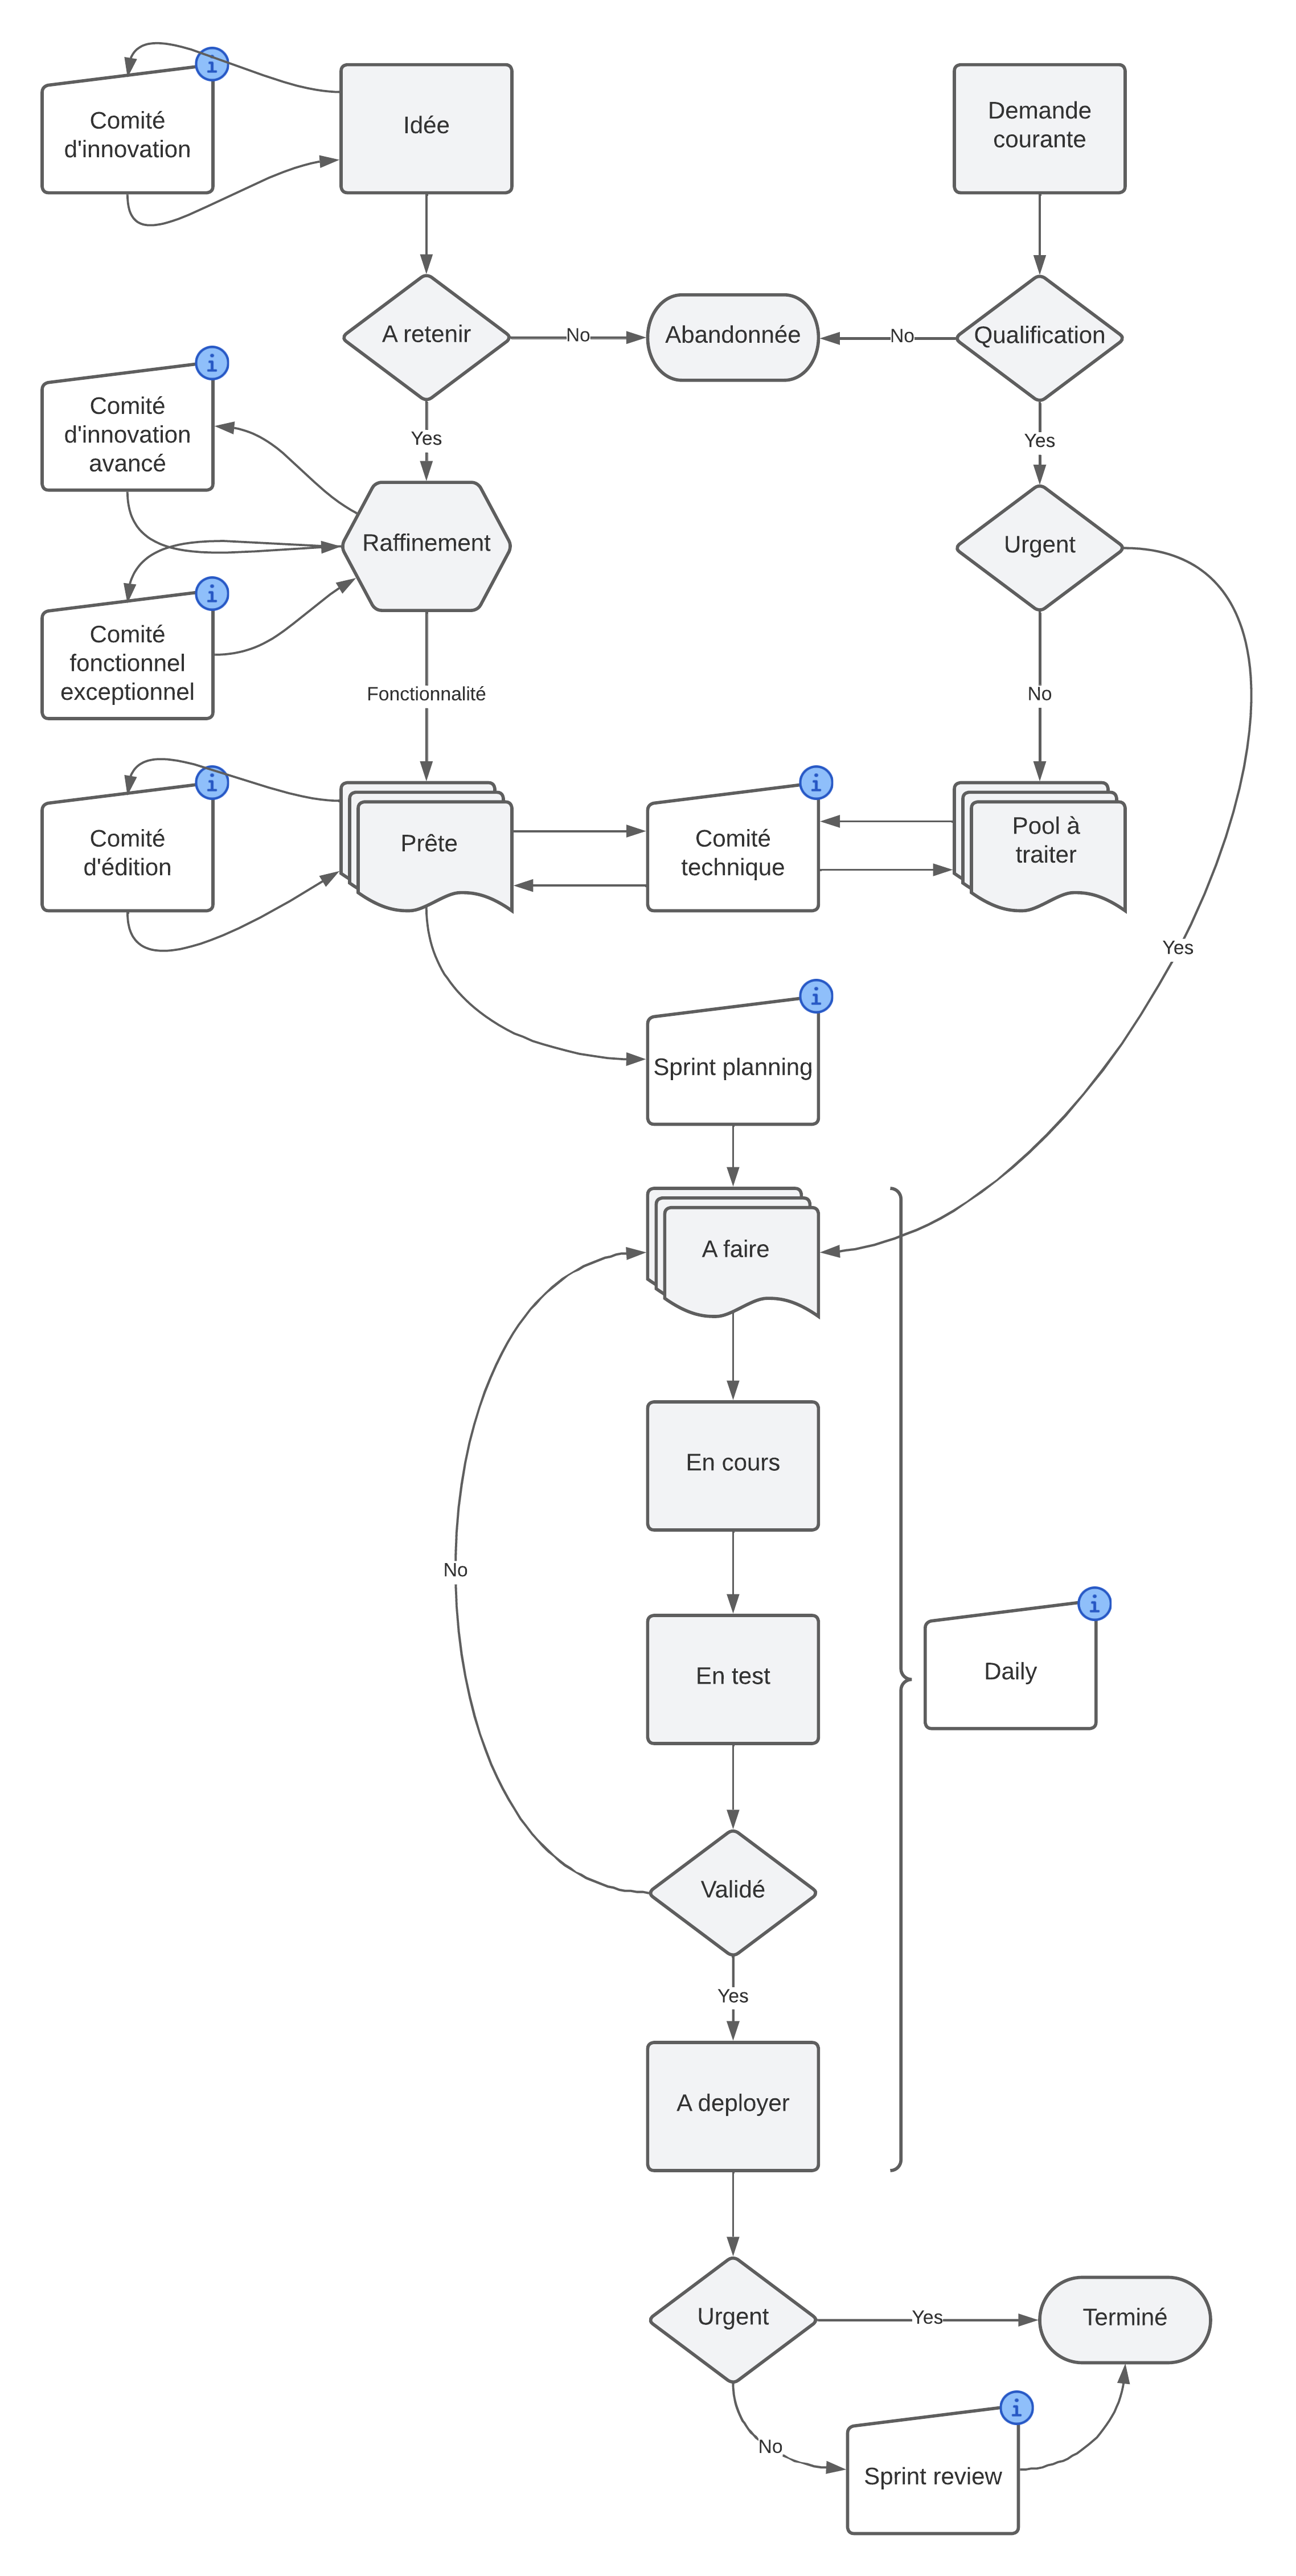
\includegraphics[height=0.94\textheight]{img/lifecycle-of-incoming-ideas}
        \caption{Diagramme d'activité du traitement des idées et des bogues (demandes courantes) entrants chez SuiviDeFlotte.}
        \label{fig:lifecycle-of-incoming-ideas}
    \end{figure}

    \begin{figure}[ht]
        \centering
        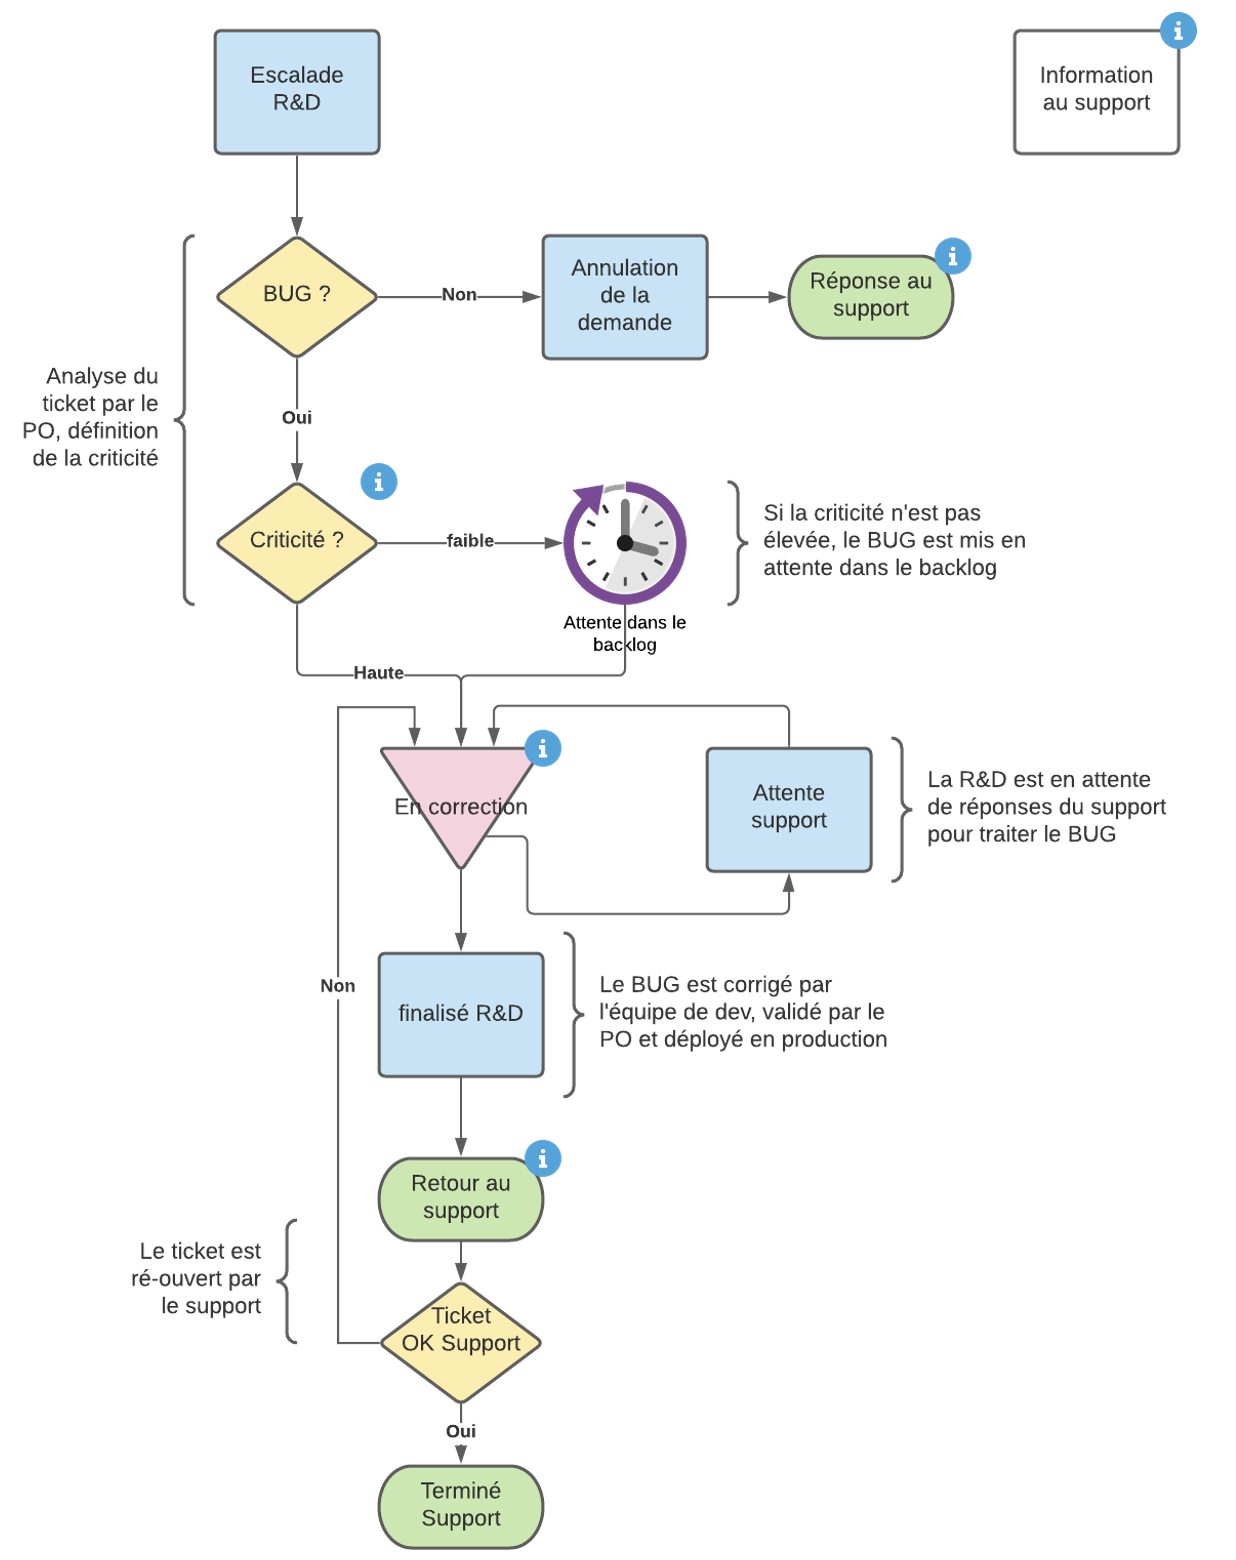
\includegraphics[width=\textwidth]{img/lifecycle-of-bugs}
        \caption{Diagramme d'activité du traitement des bogues.}
        \label{fig:lifecycle-of-bugs}
    \end{figure}

    \section{Intégration Continue et Déploiement Continu}\label{sec-a:ci-cd}

    \begin{code}
        \caption{Le fichier de configuration de Nginx (\Verb{conf.d}) du projet Pipeline documentaire utilisé en production.}
        \inputminted{nginx}{code/conf.d}
        \label{code:nginx-conf-prod}
    \end{code}

    \chapter{Pipeline Documentaire}

    \section{Les événements}

    \begin{code}
        \caption{La classe \Verb{UploadType}.}
        \inputminted{php}{code/UploadType.php}
        \label{code:upload-type}
    \end{code}

    \begin{code}
        \caption{La configuration de l'importation du fichier LCCC.}
        \inputminted{php}{code/lccc.php}
        \label{code:lccc-config}
    \end{code}

    \section{Testing}

    \begin{code}
        \caption{La classe \Verb{CheckEmailTest}.}
        \inputminted{php}{code/CheckEmailTest.php}
        \label{code:check-email-test}
    \end{code}

    \begin{code}
        \caption{Le classe \Verb{UploadControllerTest}.}
        \inputminted{php}{code/UploadControllerTest.php}
        \label{code:upload-controller-test}
    \end{code}

    \chapter{Mission frontend}

    \section{Frontend}

    \begin{code}
        \caption{La partie du fichier \Verb{.diff} téléchargé depuis GitLab qui montre le code du nouveau formulaire d'importation.}
        \inputminted[firstline=61,lastline=107]{diff}{code/frontend.diff}
        \label{code:frontend-diff-new-form}
    \end{code}

    \begin{code}
        \caption{Le code de la nouvelle fenêtre modale.}
        \inputminted[firstline=154,lastline=174]{html}{code/import.blade.php}
        \label{code:frontend-modal}
    \end{code}

    \begin{code}
        \caption{La fonction \Verb{getGuide}.}
        \inputminted[firstline=485,lastline=497]{js}{code/import.blade.php}
        \label{code:frontend-get-guide}
    \end{code}

    \begin{code}
        \caption{La fonction \Verb{importFile}.}
        \inputminted[firstline=515,lastline=547]{js}{code/import.blade.php}
        \label{code:frontend-import-file}
    \end{code}

    \begin{code}
        \caption{La fonction \Verb{importHistory}.}
        \inputminted[firstline=549,lastline=586]{js}{code/import.blade.php}
        \label{code:frontend-import-history}
    \end{code}

    \begin{code}
        \caption{La fonction \Verb{checkRecentPendingImports}.}
        \inputminted[firstline=588,lastline=596]{js}{code/import.blade.php}
        \label{code:frontend-check-recent-pending-imports}
    \end{code}

\end{appendices}